
% 3rd page
\begin{titlepage}
	
\end{titlepage}

\vspace*{\fill}
\begin{center}
	%\renewcommand{\baselinestretch}{1.5}
	{\LARGE\sffamily
		\textbf{The solar wind's geomagnetic impact and its\\Sun--Earth evolution\\--\\Predictive models for space weather\\and the Parker~Solar~Probe orbit}\\
	}
	\renewcommand{\baselinestretch}{1.5}
	
	\vspace{3\baselineskip}
	\Large\rmfamily
	Dissertation by\\
	
	\textit{Malte~S.~Venzmer}\\
	
	\vspace{2\baselineskip}
	
	\begin{minipage}{0.9\textwidth}
		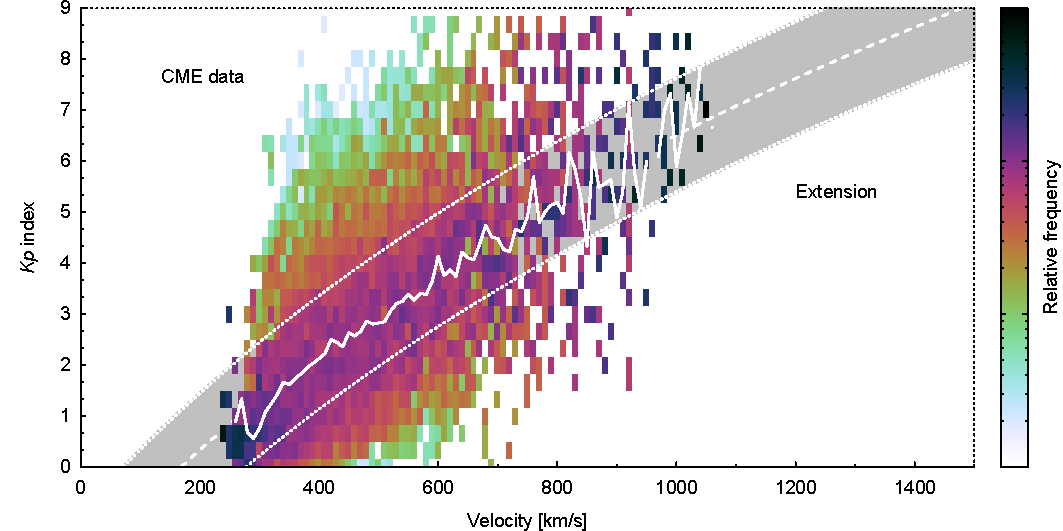
\includegraphics[width=\textwidth]{figures_of_mine/gnuplots/titlepage_plot_ch2_kpvsv_cmes_c2.pdf}
	\end{minipage}
	
	\vspace{0.5\baselineskip}
	
	\begin{minipage}{0.9\textwidth}
		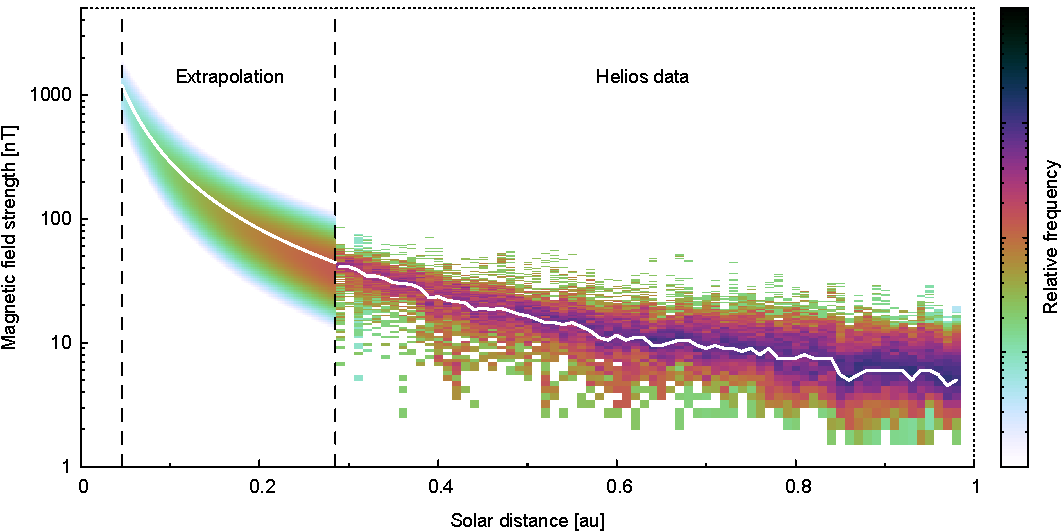
\includegraphics[width=\textwidth]{figures_of_mine/gnuplots/fit_fixed_B_paper_h_title.pdf}
	\end{minipage}
\end{center}
\vfill

\newpage

\vspace*{\fill}
\begin{small}
	\noindent \textbf{Figure on the previous page}\quad The top panel shows the relative \Kp{} frequency distribution per solar wind velocity and its mean value (solid line). The data used is based on the near-Earth OMNI data set and consists of CME-associated flows filtered with the SWS list. The derived predictive model and the mean absolute deviation are indicated by the dashed line and the gray shaded area.
	The bottom panel shows the relative frequency distribution of the solar wind magnetic field strength with respect to solar distance and its mean value (solid line). Data from the Helios probes is shown to the right and the extrapolation of the derived model to the near-Sun region is shown to the left.

	\vspace{\stretch{4}}

% 	\noindent January 2012 -- September 2018

	% 	Submitted on XX September? 2018 / Defense planned on 1 November 2018\\
	
	\vspace{1\baselineskip}
	
	\noindent 121 pages, 82 figures, 5 tables, 1 article

	\noindent Version 1.387 -- last changes \ISOToday{} \thistime{}
	
	\vspace{1\baselineskip}
	
	% electronic version note
	\noindent The electronic version of this document is fully hyperlinked. The external links in several figure captions and in the references are not accessible in the printed version. All external web links in this document were valid in 2018-09-XX.
\end{small}
\vspace{\stretch{1}}

\normalsize

% \vspace{1\baselineskip}
% 
% \begin{footnotesize}
% \noindent version log:\\
% 1	2013-11-06	created thesis.tex document\\
% % 2	2013-11-07	inserted lem excerpt\\
% % 3	2014-09-01	outlined introduction structure and appendix key words\\
% % 4	2014-09-11	bibtex included, lem excerpt citet\\
% 5	2014-09-12	included italic titles in bibliography\\
% % 6	2015-01-12	worked on introduction structure and included magnetic butterfly diagram\\
% % 7	2015-05-04	first printout, small additions\\
% % 8	2015-07-03	coupling functions, content structure\\
% % 9	2015-09-09	Alfv\'en wave velocity formula\\
% 10	2015-09-10	Appendix physics: Alfv\'en and compressional MHD waves, plasma beta; citation sources Cranmer2005, Kivelson1995\\
% % 11	2015-09-15	CGAUSS work overview; DQCS model figure\\
% % 12	2015-09-16	magnetic energy density is the same as magnetic pressure, abbreviations\\
% % 13	2015-09-30	empirical solar wind model plots in analyses, figure label [Figure 4.2  Text]\\
% % 14	2015-10-02	table column decimal alignment; set caption width\\
% % 15	2015-10-05	table units; radial parameter (N, T) profiles in literature\\
% % 16	2015-10-06	literature radial electron density models; log-normal distribution\\
% % 17	2015-10-07	log-normal formulae\\
% % 18	2015-10-08	log-normal fit\\
% % 19	2015-10-09	shape fit parameter table; radial variance fitting\\
% % 20	2015-10-14	variance fit values; log-normal citation Bronstein\\
% % 21	2015-10-19	radial distribution width fitting; clarifying of solar wind model formulae structure and naming variables\\
% % 22	2015-10-20	log-normal distribution width factor changes the shape!\\
% % 23	2015-10-23	log-normal distributions mu and sigma plot\\
% % 24	2015-10-30	new sigmafit2 figures implemented; formulae adaption\\
% % 25	2015-11-02	reason for use of log-normal function\\
% % 26	2015-11-20	single log-normal shape fit; not chisquare - SSR; $R^2$ in appendix\\
% % 27	2015-11-26	reduced SSR into tables; table column aligning\\
% % 28	2015-12-02	smoothing SSR integration\\
% % 29	2015-12-07	integrating structure remarks from printout\\
% % 30	2015-12-09	splitting analyses chapter into two; browsing folders for usable things for thesis\\
% % 31	2015-12-10	integrating citations and references\\
% % 32	2015-12-16	integrating citations and references\\
% % 33	2015-12-18	solar wind structures list of Richardson\\
% % 34	2016-02-02	sws distributions\\
% % 35	2016-02-11	basics structure\\
% % 36	2016-02-12	analyses questions\\
% % 37	2016-02-15	analyses structure; in situ, near-Sun\\
% % 38	2016-02-16	Kp index internal resolution\\
% % 39	2016-02-17	Bartels1962; non-breaking hyphen shorthand implemented\\
% % 40	2016-02-18	analysesI structure\\
% % 41	2016-02-25	abstract\\
% % 42	2016-02-26	english comma\\
% % 43	2016-03-01	Bartels Kp origin paper, bibtex reference\\
% % 44	2016-03-02	abstract\\
% % 45	2016-03-03	Planck paper\\
% % 46	2016-03-07	formation of stars\\
% % 47	2016-03-08	formation of stars\\
% % 48	2016-03-16	solar interior structure\\
% % 49	2016-03-17	solar interior structure\\
% 50	2016-03-18	solar surface\\
% % 51	2016-03-22	Astronomical Almanac citation\\
% % 52	2016-03-23	solar core definition\\
% % 53	2016-03-26	sunspots\\
% % 54	2016-03-29	Sun interior figure\\
% % 55	2016-03-30	solar composition\\
% % 56	2016-03-31	Sun interior figure finished; chromosphere\\
% % 57	2016-04-01	Sun atmosphere figure finished\\
% % 58	2016-04-03	chromosphere, corona, CV\\
% % 59	2016-04-07	CV\\
% % 60	2016-04-08	CV; heliosphere\\
% % 61	2016-04-09	corona; heliosphere\\
% % 62	2016-04-11	heliosheath magnetic bubbles; Opher2011\\
% % 63	2016-04-12	heliosphere; voyagers; Gurnett2013\\
% % 64	2016-04-13	solar wind effects, solar rotation\\
% % 65	2016-04-14	analysesI sws structure draft plots\\
% % 66	2016-04-15	analysesI concept work\\
% % 67	2016-04-19	incorporate annotations from processed printout\\
% % 68	2016-04-21	incorporate annotations from processed printout II\\
% % 69	2016-04-22	incorporate annotations from processed printout III\\
% % 69	2016-04-23	updated .bst file (for displaying arXiv id); implemented optional url displaying for electronic version; Kp year variations\\
% % 70	2016-04-24	Kp frequency by month statistics and plot; Sun and Earth tilt plot\\
% % 71	2016-04-25	solar cycle extrema dates literature\\
% % 72	2016-04-27	Kp semi annual variation, Rangarajan1997\\
% % 73	2016-05-01	Kp frequency by year\\
% % 74	2016-05-04	Kp + SSN plot; ACE data errors/gaps; log-normal plot; differential rotation plot\\
% % 75	2016-05-05	aggregate correlation coefficient tables, CME fraction plot\\
% % 76	2016-05-06	overall sws fractions\\
% % 77	2016-05-17	figure sw frequencies by year; restructured solar wind distributions section; formal cover page\\
% % 78	2016-05-20	Earth-Sun distance; JPL web interface\\
% % 79	2016-05-31	GSM system\\
% % 80	2016-06-10	Offline Anmerkungen einarbeiten\\
% % 81	2016-06-12	LaTeX Earth symbol package\\
% % 82	2016-06-13	numbers=noenddot\\
% % 83	2016-06-14	references removed comma before ampersand; offline Anmerkungen einarbeiten; thesis\_raw version\\
% % 84	2016-06-17	gnuplot figures and latex; latex document style options\\
% % 85	2016-06-19	header implemented\\
% % 86	2016-06-20	minor things; introduction\\
% % 87	2016-06-23	solar tilt axis\\
% % 88	2016-06-24	solar rotation\\
% % 89	2016-07-12	magnetosphere temp figure; analyses: solar wind model\\
% % 90	2016-07-13	lognormal spelling\\
% % 91	2016-07-14	constant mass flow rate\\
% % 92	2016-07-18	line-up periods\\
% % 93	2016-07-19	line-up periods table\\
% % 94	2016-07-20	redone line-up analysis\\
% % 95	2016-07-21	line-up tables\\
% % 96	2016-07-22	line-up fit function plots; coefficient table\\
% % 97	2016-07-22	line-up sw types and period plots; overview plot\\
% % 98	2016-07-24	line-up averaging and justification\\
% % 99	2016-07-29	line-up rework\\
% 100	2016-07-30	line-up structure\\
% % 101	2016-07-31	line-up table\\
% % 102	2016-08-02	line-up structure\\
% % 103	2016-08-03	line-up fits and table\\
% % 104	2016-08-04	insert offline comments\\
% % 105	2016-08-15	literature radial sw functions\\
% % 106	2016-08-18	work offline comments in\\
% % 107	2016-08-19	work offline comments in\\
% % 108	2016-08-28	analyses II rework structure\\
% % 109	2016-08-31	analyses II rework structure\\
% % 110	2016-09-01	analyses II rework figures\\
% % 111	2016-09-02	analyses II rework structure\\
% % 112	2016-09-03	Helios latitude dependency\\
% % 113	2016-09-04	extrapolation model fit parameter table; Helios latitude dependence\\
% % 114	2016-09-06	work in offline comments\\
% % 115	2016-09-14	implement median and mean in composite fit table; create kile project for thesis; url and raw fork\\
% % 116	2016-09-17	Ulysses polar plot; solar distance plots\\
% % 117	2016-09-18	for solar distance and latitude -> 4-panel figures created and implemented; appendix figures\\
% % 118	2016-09-20	latitude plots updated\\
% % 119	2016-09-26	single lognormal fit figure\\
% % 120	2016-09-27	minor tweaks in analyses II\\
% % 121	2016-09-29	simple fit table errors; table style\\
% % 122	2016-10-05	lognormal fit errors for tables\\
% % 123	2016-10-10	line-up passing remarks from AP\\
% % 124	2016-10-12	siunitx package incorporated\\
% % 125	2017-01-04	package fancyhdr replaced with scrlayer-scrpage; offline comments for Basics + Data incorporated\\
% % 126	2017-01-06	package floatrow included for figure side captions; some cites; magnetometer\\
% % 127	2017-01-08	sun figure updates and new ion energy spectrum figure incorporated\\
% % 128	2017-01-13	offline comments, new chapter order\\
% % 129	2017-01-18	activated hyperref package; included autoref and eqref; adjusted link colors; header links\\
% % 130	2017-02-02	offline commtents\\
% % 131	2017-02-03	offline commtents II, eclipse image\\
% % 132	2017-02-06	basics figures with floatrow; flow structure\\
% % 133	2017-02-07	ion energy spectrum figure\\
% % 134	2017-02-09	Helios mission ssn plot\\
% % 135	2017-02-12	offline comments\\
% % 136	2017-02-13	section number link to toc; offline comments\\
% % 137	2017-02-14	eclipse and magbfly figure captions\\
% % 138	2017-02-16	offline comments\\
% % 139	2017-02-19	coronal heating and sw acceleration\\
% % 140	2017-04-22	set up git repository\\
% % 141	2017-04-23	incorporate offline comments\\
% % 142	2017-04-26	bipolar region draft\\
% % 143	2017-04-27	magnetic layer Ossendrijver2003\\
% % 144	2017-06-29	magnetosphere figure drafts implemented\\
% % 145	2017-07-16	streamlined content - including paper and chapter2\\
% % 146	2017-07-22	streamlined duplicate content\\
% % 147	2017-10-05	Kp index data\\
% % 148	2017-10-28	geomagnetic indices; Kp index; Kp to ap table\\
% % 149	2017-10-29	Kp index\\
% 150	2017-10-30	OMNI s/c coverage figure\\
% % 151	2017-10-31	OMNI s/c coverage figure upgrade; data set timeline figure\\
% % 152	2017-11-01	SSN prediction; omega-effect\\
% % 153	2017-11-02	alpha-omega dynamo; magnetogram figure upgrade\\
% % 154	2017-11-03	worked on figure permissions; alpha-omega-figure\\
% % 155	2017-11-04	paperMVVB inserted; worked on compatibility\\
% % 156	2017-11-12	paperMVVB: figure size, tablefoot, adjusted table width; included chapter2; ordered file implementing\\
% % 157	2017-11-14	figure permission Babaszkiewicz1998\\
% % 158	2017-11-15	poking around in image credits; solar activity cycle\\
% % 159	2017-11-16	solar activity cycle; Zhao image permission\\
% % 160	2017-11-17	Zhao copyright symbol included; solar wind; commata and sentence wording\\
% % 161	2017-11-22	notes from github paper folder\\
% % 162	2017-11-23	Ulysses figure permission and caption; pdfpages package; paper included as is\\
% % 163	2017-11-24	GUM reference; Helios data frequency figure\\
% % 164	2017-11-25	intro to paper\\
% % 165	2017-11-26	intro to paper\\
% % 167	2017-11-27	Cranmer2005 fig1; Banaszkiewicz fig\\
% % 168	2017-11-28	HCS and Parker spiral\\
% % 169	2017-11-29	heliosheath; Cranmer2005 permission\\
% % 170	2017-11-30	chapter2 updated\\
% % 171	2017-12-06	upgraded: title, abstract, introduction, basics outline, notes to chapter2; worked in offline comments until HMF\\
% % 172	2017-12-08	MBPs; Solar wind section structure\\
% % 173	2017-12-10	solar wind basics, draft figs for CIR and CME\\
% % 174	2017-12-11	draft figs for COR2 CME and ACE MC; solar wind history\\
% % 175	2017-12-13	B-field improvement\\
% % 176	2017-12-14	B-field improvement \#2\\
% % 177	2017-12-15	B-field improvement \#3\\
% % 178	2017-12-16	B-field angles plot\\
% % 179	2017-12-17	B-field improvement \#4\\
% % 180	2017-12-21	B-field: four plots upgraded\\
% % 181	2017-12-31	B-field: worked offline comments in; included chapter2 update\\
% % 182	2018-01-01	autoref names; solar wind properties; literature\\
% % 183	2018-01-02	sw helium share; plasma beta; source surface; mass flux considerations\\
% % 184	2018-01-04	sw considerations; fast/slow wind\\
% % 185	2018-01-05	fig Hundhausen; fast slow sw\\
% % 186	2018-01-08	fast slow sw\\
% % 187	2018-01-09	slow sw sources\\
% % 188	2018-01-10	slow sw; slow/fast cycle pattern\\
% % 189	2018-01-11	Wang1990\\
% % 190	2018-01-14	HCS and SIR\\
% % 191	2018-01-15	HCS + CIR\\
% % 192	2018-01-16	in-situ event plots\\
% % 193	2018-01-17	in-situ CIR/HSS plot\\
% % 194	2018-01-19	CME/MC plot; VB comments\\
% % 195	2018-01-20	VB comments...\\
% % 196	2018-01-21	VB comments; Alfvén waves\\
% % 197	2018-01-22	VB comments; removed line-up study; merged appendix; removed unused tex and image files\\
% % 198	2018-01-24	HMF offline comments\\
% % 199	2018-01-26	B improvement offline comments; APL PSP pictures; adjust pdfinfo\\
% 200	2018-01-28	chapter2 implemented into thesis; figure folders rearranged; figures floatrow implemented\\
% % 201	2018-01-29	abstract updated; contents structure streamlined\\
% % 202	2018-01-29b	instrumentation and data sources\\
% % 203	2018-01-30	OMNI and Helios data\\
% % 204	2018-01-31	chapter2 R-M effect literature\\
% % 205	2018-01-31b	R-M effect literature; chapter2 coupling into basics\\
% % 206	2018-02-01	formal titlepage\\
% % 207	2018-02-03	front matter; pdf toc bookmarks\\
% % 208	2018-02-05	sw in-situ fig\\
% % 209	2018-02-06	SIRs\\
% % 210	2018-02-07	SIRs II\\
% % 211	2018-02-09	CMEs\\
% % 212	2018-02-11	CMEs II\\
% % 213	2018-02-11b	CMEs IIb\\
% % 214	2018-02-12	CMEs III\\
% % 215	2018-02-13	CMEs IV\\
% % 216	2018-02-14	CMEs V\\
% % 217	2018-02-15	CMEs VI\\
% % 218	2018-02-16	CME images...\\
% % 219	2018-02-19	HCS into HMF\\
% % 220	2018-02-20	HCS in sw section\\
% % 221	2018-02-21	work in offline comments\\
% % 222	2018-02-23	work in offline comments II\\
% % 223	2018-02-25	CMEs; CMEs.tex\\
% % 224	2018-02-26	CMEs.tex II\\
% % 225	2018-02-27	CMEs.tex III\\
% % 226	2018-02-28	figure captions - removed explanations\\
% % 227	2018-03-01	figure permissions documentation 80\%\\
% % 228	2018-03-02	figure permissions list - remove caption before credits; CMEs.tex IV\\
% % 229	2018-03-03	CMEs.tex V\\
% % 230	2018-03-04	CMEs.tex VI, BSS\\
% % 231	2018-03-04b	CMEs.tex VI, MC figure\\
% % 232	2018-03-05	CMEs.tex VII, CBS\\
% % 233	2018-03-05b	CMEs.tex VIIb, 3D models\\
% % 234	2018-03-06	CMEs, figures\\
% % 235	2018-03-07	CMEs, figures, fig. captions\\
% % 236	2018-03-08	CMEs.\\
% % 237	2018-03-09	CMEs..\\
% % 238	2018-03-10	figure permission hundhausen1977\\
% % 239	2018-03-13	CME formation\\
% % 240	2018-03-16	chapter2 offline corrections implemented\\
% % 241	2018-03-17	chapter2 fit curves figure; sw example plot vBz figure\\
% % 242	2018-03-19	chapter2 sw example plot v figure; and figure captions\\
% % 243	2018-03-20	new paper pdf; references link shortcuts\\
% % 244	2018-03-21	chapter2 SSN 300 plots corrected; error sizes; quantiles added; CME offline corrections\\
% % 245	2018-03-22	CME offline corrections; magnetosphere figure...\\
% % 246	2018-03-25	last CME offline corrections; paper B-field addendum offline corrections\\
% % 247	2018-03-26	CME formation; space weather\\
% % 248	2018-03-28	stuff from Cranmer2017, Savani2015+2017\\
% % 249	2018-03-29	magnetosphere figure implemented\\
% 250	2018-03-31	Adams comments for PSP chapter; sectioning space weather + magnetosphere\\
% % 251	2018-04-01	magnetosphere 2D and 3D figures; DeKeyser2005 + Phan2005; Dungey1963\\
% % 252	2018-04-03	space\_weather.txt 1--3\\
% % 253	2018-04-04	space\_weather.txt 4\\
% % 254	2018-04-05	electronic version note; space\_weather.txt implemented; excerpts sorted\\
% % 255	2018-04-06	Dungey cycle\\
% % 256	2018-04-06b	Summary\\
% % 257	2018-04-07	magnetosphere sorting\\
% % 258	2018-04-09	space weather\\
% % 259	2018-04-10	space weather 2; magnetosphere\\
% % 260	2018-04-11	magnetosphere 3; reconnection figure\\
% % 261	2018-04-16	CMEs; showoff version created\\
% % 262	2018-04-16b	title figure 2\\
% % 263	2018-04-19	space weather offline comments incorporated\\
% % 264	2018-04-20	coupling mechanisms\\
% % 265	2018-04-21	coupling mechanisms; turbulence\\
% % 266	2018-04-22	Dungey cycle\\
% % 267	2018-04-23	Dungey cycle 2\\
% % 268	2018-04-24	Dungey cycle 3\\
% % 269	2018-04-25	Dungey cycle 4\\
% % 270	2018-04-25b	R-M effect\\
% % 271	2018-04-26	R-M effect 2\\
% % 272	2018-04-26b	geomagnetic storms\\
% % 273	2018-04-30	geomagnetic storms 2\\
% % 274	2018-05-01	offline comments s/w; stream kp-sw plot\\
% % 275	2018-05-02	geomagnetic storms 3\\
% % 276	2018-05-03	geomagnetic storms 4; Dst index\\
% % 277	2018-05-04	not really\\
% % 278	2018-05-05	Birkeland current system\\
% % 279	2018-05-07	offline comments implemented\\
% % 280	2018-05-08	kp index\\
% % 281	2018-05-09	minor changes\\
% % 282	2018-05-09	Geomagnetic activity forecast; E = -vBz\\
% % 283	2018-05-10	E = -vBz\\
% % 284	2018-05-11	coupling functions; Newell function\\
% % 285	2018-05-12	coupling functions\\
% % 286	2018-05-13	coupling functions 3\\
% % 287	2018-05-14	coupling functions 4\\
% % 288	2018-05-17	implementing offline comments: coupling functions\\
% % 289	2018-05-30	coupling functions 5\\
% % 290	2018-05-31	Kp forecast\\
% % 291	2018-06-01	implementing offline comments: Kp forecast\\
% % 292	2018-06-02	implementing offline comments 2: coupling functions\\
% % 293	2018-06-03	Kp empirical functions\\
% % 294	2018-06-04	Kp empirical functions 2\\
% % 295	2018-06-05	Wing Kp model\\
% % 296	2018-06-07	prediction performance and true skill score\\
% % 297	2018-06-10	appendix: true skill statistics\\
% % 298	2018-06-11	appendix: true skill statistics; Kp persistence\\
% % 299	2018-06-12	chapter2: prediction performance, TSS, statistics table\\
% 300	2018-06-13	chapter2: TSS\\
% % 301	2018-06-14	Kp forecast models\\
% % 302	2018-06-16	comments Adam + VB\\
% % 303	2018-06-17	comments VB\\
% % 304	2018-06-17b	comments VB 2\\
% % 305	2018-06-18	comments VB 3\\
% % 306	2018-06-19	Kp forecast; CME forecast\\
% % 307	2018-06-20	Kp prediction models\\
% % 308	2018-06-21	magnetometer\\
% % 309	2018-06-22	sw forecast to Earth\\
% % 310	2018-06-23	acknowledgements; coordinate systems\\
% % 311	2018-06-25	coordinate systems\\
% % 312	2018-06-26	magnetometer; plasma detector\\
% % 313	2018-06-27	lognormal distribution; Sun-Earth geometry\\
% % 314	2018-06-27b	Sun-Earth geometry plot; solar distance\\
% % 315	2018-06-28	Sun-Earth geometry 2\\
% % 316	2018-06-28b	plasma detector 2\\
% % 317	2018-06-29	solar differential rotation\\
% % 318	2018-06-29b	solar differential rotation 3\\
% % 319	2018-06-30	sw stream and CME forecast to Earth\\
% % 320	2018-06-30b	sw stream and CME forecast to Earth 2\\
% % 321	2018-07-01	looking through chapter2 until 4.3\\
% % 322	2018-07-01b	looking through chapter2 until 4.3.2; E-field at the magnetopause\\
% % 323	2018-07-02	looking through chapter2 until 4.3.3\\
% % 324	2018-07-02b	looking through chapter2 until 4.4\\
% % 325	2018-07-04	offline comments implemented\\
% % 326	2018-07-04b	offline comments implemented 2\\
% % 327	2018-07-05	last offline comments, CME forecast\\
% % 328	2018-07-09	data links into text; CME forecast 2\\
% % 329	2018-07-10	solar wind nowcast; looking through chapter2 until 4.4.1\\
% % 330	2018-07-11	looking through chapter2 until 4.4.3\\
% % 331	2018-07-12	looking through chapter2\\
% % 332	2018-07-13	PSP mission\\
% % 333	2018-07-14	introduction\\
% % 334	2018-07-16	implement offline comments\\
% % 335	2018-07-17	PSP mission 2; acronyms\\
% % 336	2018-07-19	english titlepage; tabular CV; minor things\\
% % 337	2018-07-20	acronyms into two columns; chapterPSP\\
% % 338	2018-07-21	chapterPSP; figure: IMF comparison\\
% % 339	2018-07-22	chapterPSP\\
% % 340	2018-07-22b	chapterPSP discussion\\
% % 341	2018-07-23	basics intro; introduction synopsis\\
% % 342	2018-07-25	implement offline comments chapterPSP; tabular CV\\
% % 343	2018-07-25b	acknowledgments\\
% % 344	2018-07-28	implement offline comments chapter2\\
% % 345	2018-07-28b	implement offline comments chapter2 2; summary handout\\
% % 346	2018-07-29	implement offline comments appendix ff.\\
% % 347	2018-07-30	abstract page\\
% % 348	2018-07-30b	introduction\\
% % 349	2018-07-31	introduction 2\\
% 350	2018-08-01	data acknowledgments\\
% % 351	2018-08-01b	introduction 3\\
% % 352	2018-08-02	introduction 4\\
% % 353	2018-08-03	introduction 5\\
% % 354	2018-08-05	introduction 6\\
% % 355	2018-08-06	new title; conclusions\\
% % 356	2018-08-08	implement offline comments chapter2\\
% % 357	2018-08-09	implement offline comments chapter2 2\\
% % 358	2018-08-13	comments Tal introduction\\
% % 359	2018-08-14	implement offline comments chapter2 b\\
% 360	2018-08-15	chapter2 rework sw figures\\
% % 361	2018-08-16	chapter2 discussion + conclusions\\
% % 362	2018-08-17	chapter2 discussion + conclusions 2\\
% % 363	2018-08-18	chapterPSP; figure placement data+appendix; list of figure permissions\\
% % 364	2018-08-20	chapter2 conclusions; chapterPSP flux conservation\\
% % 365	2018-08-21	chapterPSP sw model refinements; conclusions synopsis\\
% % 366	2018-08-22	CV minor\\
% % 367	2018-08-23	work on 1st full version: abstract; remove notes; chapter2 conclusions; overhanging lines\\
% % 368	2018-08-24	conclusions: ch2 summary+results\\
% % 369	2018-08-24b	conclusions: ch2 conclusions\\
% 370	2018-08-25	ch2: both sw plots 9hshift + extension plot + 3rd page plot \#2\\
% % 371	2018-08-26	3rd page plot \#1 + figure description + page layout; conclusions chPSP\\
% % 372	2018-08-28	implement offline comments; conclusions: chPSP\\
% % 373	2018-08-28b	conclusions: chPSP summary\\
% % 374	2018-08-29	conclusions: chPSP results\\
% 375	2018-08-29b	conclusions: chPSP conclusions\\
% 376	2018-08-30	outlook\\
% 377	2018-08-31	conclusions minor changes; GN's introduction comments\\
% 378	2018-09-01	committee member order; 3rd page layout\\
% 379	2018-09-03	Tal comments basics + chapter2; spell check thesis\\
% 380	2018-09-05	comments GN conclusions; implemented new abstract\\
% 381	2018-09-06	notes integrated: introduction + chapter2 + conclusions\\
% 382	2018-09-07	introduction; figure placement: Basics + chapter2\\
% 383	2018-09-08	figure placement and pagebreaks: rest of document; new figures: introduction: CME + PSP, basics: WSA-Enlil, chapterPSP: PSP with third stage;removed spacing in references\\
% 384	2018-09-09	comments Tal conclusions; search language word misuses/errors in whole document\\
% 385	2018-09-10	conclusions update\\
% 386	2018-09-11	GN comments abstract; acronym check\\
% 387	2018-09-12	test links: 3 defunct\\
% \vspace{\baselineskip}
% \ISOToday{} \thistime{} -- last save
% \end{footnotesize}


\clearpage

\normalsize

\vspace*{\fill}

%Zitat in Diplomarbeit:
%\textit{"[...], und während er sich solchermaßen in der unteren Region des Reiches der Wissenschaft bewegte, dort, wo dieses unmerklich in das Reich der Psychiater übergeht, eignete er sich schließlich doch eine ganze Menge durchaus nützlicher Kenntnisse an, [...]"}
%denn er wusste immer erstaunlich gut Bescheid,
%\noindent Zitat: Stanislaw Lem, "Die Stimme des Herrn", S.56.

\noindent \textit{``Despite the `Dr.' before his name, he had completed no course of study and received no degree. When people tried to pin him down about this, he would say that the letters were merely an abbreviation of his first name - Drummond - which he did not use. But it was as `Dr.' Sam Laserowitz that he appeared in a number of science-fiction magazines; he was also known, in the circles of the fans of that genre, as a lecturer, and spoke on `cosmic' themes at their many conferences and convention. Laserowitz's speciality was earthshaking discoveries, wich he happened upon two or three times a year. [...] We really have no idea what a multitude of con men and crackpots inhabit the domain that lies halfway between contemporary science and the insane asylum.''}
\vspace{\baselineskip}

\noindent Excerpt from Stanis\l aw Lem 1968, \textit{His Master's Voice} \citep[p.~38]{Lem1984}.
%quote vs quotation vs excerpt

% \vspace{\stretch{2}}
% 
% \noindent \textit{``Asking for the average solar wind might appear as silly as asking for the taste of an average drink. What is the average between wine and beer? Obviously mere mixing -- and averaging means mixing -- does not lead to a meaningful result. Better taste and judge separately and then compare, if you wish. After a while you will have developed a set of criteria for differentiating. Then you may eventually come from analysis to synthesis: You really can appreciate what you are drinking. So much for the drinks.''}
% \vspace{\baselineskip}
% 
% \noindent Excerpt from Rainer Schwenn 1983, \textit{The 'average' solar wind in the inner heliosphere: Structures and slow variations} \citep[introduction]{Schwenn1983}.

\vfill

\cleardoublepage

\begin{titlepage}
 
\end{titlepage}

% \begin{abstract}
\begin{center}
	{\LARGE \sffamily \textbf{Abstract}}	%or abstract=true
\end{center}
This thesis addresses two current topics in solar wind research and space weather. The first study is dedicated to the solar wind's impact on geomagnetic activity and the second study to the estimation of the solar wind conditions in the near-Sun environment with regard to the Parker Solar Probe mission.

\medskip

% \noindent \textit{Context.}
Solar wind interacts with the terrestrial magnetosphere, and variations in its properties result directly in geomagnetic disturbances. Extreme plasma conditions, such as those found exclusively found in coronal mass ejections (CMEs), evoke geomagnetic storms that can potentially disrupt technological systems and pose threats to human lives. Therefore, the prediction of space weather effects is of major importance.
% \noindent \textit{Aims.}
This study aims to derive empirical relations in order to predict the planetary geomagnetic disturbance indicator \Kp{} from the solar wind electric field and from the velocities of CMEs and solar wind streams.

% \noindent \textit{Methods.}
Near-Earth solar wind measurements of the period 1981--2016 from the minutely OMNI data set are processed to 3"~hourly averages and to 3"~hourly extrema, and correlated with the \Kp~index. A functional dependency between \Kp{} and the electric field proxy \vBz{} in GSM coordinates is derived. CME and stream data are separated using the existing list of Solar Wind Structures, and functional \Kp{} dependencies are derived for their velocities. The obtained relations are evaluated for their prediction performance by calculating forecast errors and true skill scores.
% \noindent \textit{Results.}
The \Kp{} correlation with 3"~hour minima of \vBz{} results in a significantly larger coefficient ($r_\text{min} = 0.72$) than with 3"~hour averages ($r_\text{avg} = 0.36$), whereas the correlation coefficients for 3"~hour maxima and averages of the velocity remain similar. Predictive \Kp{} models are obtained based on relations with the solar wind electric field, and the velocity of CMEs and streams -- the relations show mean absolute deviations of around 1~\Kp~value. The curve of the CME velocity relation is higher in magnitude and steeper in trend than that for the stream velocity. The extension of the CME velocity relation shows that CMEs with about \SI{1500}{\km\per\s} generate the maximum \Kp{} of \num{9.0}, the fastest streams with \SI{900}{\km\per\s} however, barely reach the geomagnetic storm threshold of $\text{\Kp} = 5.0$.
% \noindent \textit{Conclusions.}
The results suggest that by using the \vBz{} minima over 3~hours, short-term geoeffective magnetic features in the solar wind are being accounted for, which are being neglected when calculating 3"~hour averages. The evident differences in the CME and stream velocity dependencies support the approach of deriving separate \Kp{} models for them. Within their proper \Kp{} ranges, all three predictive models perform significantly better than random, and outside they still track the general trend within \Kp{} errors of about \num{+-3}.

\medskip

% \noindent \textit{Context.}
Up to now, multiple space probes have measured the solar wind in-situ throughout the whole range of the heliosphere, except for the region close to the Sun below solar distances of \SI{0.28}{\au}. Yet, this region is of particular interest as it comprises the processes that heat and accelerate the solar wind. The Parker Solar Probe (PSP) mission is the first spacecraft to visit this unexplored near-Sun region. Launched in August 2018, PSP is giong to reaches its first perihelion at a solar distance of \SI{35.7}{\Rs} (\SI{0.16}{\au}) in November 2018 and its first closest at \SI{9.86}{\Rs} (\SI{0.046}{\au}) in December 2024.
% \noindent \textit{Aims.}
This study aims to develop a solar wind model for the inner heliosphere and to predict the near-Sun solar wind environment for the PSP orbit.

% \noindent \textit{Methods.}
The model comprises individual relations that represent the frequency distributions of the solar wind key properties magnetic field strength, proton velocity, density, and temperature. The relations are constructed in such a way that the distributions are being shifted depending on solar activity and solar distance. The frequency distributions are obtained from 53~years (1963--2016) of near-Earth solar wind measurements from the hourly OMNI data set. Their shapes are fitted with lognormal functions -- the velocity is fitted with a double lognormal function to account for its slow and fast wind components. The distributions' shifts due to solar activity are derived from the monthly sunspot number (SSN) of almost five solar cycles. The velocity is treated differently in that the two lognormal functions are being balanced according to the SSN. The distributions' dependencies on solar distance are based on solar wind measurements made in the solar distance range \SIrange{0.29}{0.98}{\au} by the Helios~1 and Helios~2 spacecraft which flew in the 1970s. The dependencies are based on power-law functions, fitted to the Helios data. For the magnetic field strength, an alternative distance dependency is derived, which accounts for the Parker geometry of the individual field components. The derived solar wind model is extrapolated, using SSN predictions of the next solar cycle, down to the orbital trajectory of PSP, in particular to its first perihelion and to its first closest perihelion.
% \noindent \textit{Results.}
The estimated median values at PSP's first and first closest perihelia are respectively: \SI{87}{\nano\tesla} and \SI{943}{\nano\tesla}, \SI{340}{\km\per\s} and \SI{290}{\km\per\s}, \SI{214}{\per\cm\cubed} and \SI{2951}{\per\cm\cubed}, \SI{5.03e5}{\kelvin} and \SI{1.93e6}{\kelvin}. The median values for the magnetic field strength based on the Parker field geometry are \SI{94}{\nano\tesla} and \SI{1241}{\nano\tesla}, which is \SI{8}{\%} and \SI{32}{\%} higher than those from the model based on the power-law distance dependency. These estimates agree with those from studies using direct measurements obtained from remote observations, except for the velocity and temperature values below \SI{20}{\Rs}, which are extrapolated to be significantly higher.
% \noindent \textit{Conclusions.}
As it is known that the magnetic field strength in the outer heliosphere conforms to the Parker field geometry, the predictions of this model are considered to be more reliable. The overestimation of the near-Sun velocity and temperature values below \SI{20}{\Rs} indicates that the solar wind is still being heated and accelerated in this region.

% \end{abstract}

% \noindent Key words: solar wind -- coronal mass ejections (CMEs) -- solar-terrestrial relations -- magnetosphere -- \Kp~index -- inner heliosphere -- Parker Solar Probe (PSP)

\newpage

%\cleardoublepage
%\tableofcontents
\pdfbookmark[0]{Contents}{toc_pdf_bookmark}
{\let\cleardoublepage\clearpage\tableofcontents}	%open contents on left page
\label{sec:toc}
\cleardoublepage
%\listoffigures
%\listoftables

